% =====================================================================
% MATH-454 Parallel and High Performance Computing -- Final project
% Report: Lattice Boltzmann 2D flow past a cylinder (MPI + CUDA)
% Clean two-column A4 article template.
% Build: pdflatex report.tex  (run twice for references)
% =====================================================================
\documentclass[10pt,twocolumn,a4paper]{article}

% --- Page geometry: tight, clean A4 margins ---
\usepackage[a4paper,margin=1.8cm,columnsep=0.7cm]{geometry}

% --- Encoding and fonts ---
\usepackage[utf8]{inputenc}
\usepackage[T1]{fontenc}
\usepackage{lmodern}

% --- Math, graphics, tables ---
\usepackage{amsmath,amssymb}
\usepackage{graphicx}
\usepackage{booktabs}
\usepackage[hidelinks]{hyperref}
\usepackage{caption}
\captionsetup{font=small,labelfont=bf}

% --- Headings a bit tighter ---
\usepackage{titlesec}
\titlespacing*{\section}{0pt}{1.2ex}{0.6ex}
\titlespacing*{\subsection}{0pt}{0.8ex}{0.4ex}

\graphicspath{{../plotting/figures/}}

% --- Title ---
\title{\vspace{-1.2em}\textbf{Lattice Boltzmann Method: 2D Flow Past a Cylinder\\
\large Parallelisation with MPI and CUDA, and a Performance Study}}
\author{Simon Pierre \\ \small MATH-454 -- Parallel and High Performance Computing}
\date{\small June 2026}

\begin{document}
\maketitle

% =====================================================================
\section{Introduction and method}
% =====================================================================
The Lattice Boltzmann Method (LBM) solves fluid flow by tracking nine
particle populations $f_i(\mathbf{x},t)$ per cell on a regular D2Q9
grid, one per discrete velocity $\mathbf{c}_i$. The macroscopic density
and velocity are recovered as $\rho=\sum_i f_i$ and
$\rho\mathbf{u}=\sum_i \mathbf{c}_i f_i$. Each time step applies two
operations. \emph{Collision} (BGK) relaxes every cell towards the local
equilibrium with a single relaxation time $\tau$,
\begin{equation}
  f_i \leftarrow f_i - \tfrac{1}{\tau}\,(f_i - f_i^{\mathrm{eq}}),
\end{equation}
with $f_i^{\mathrm{eq}} = w_i\,\rho\,(1+3\,\mathbf{c}_i\!\cdot\!\mathbf{u}
+\tfrac{9}{2}(\mathbf{c}_i\!\cdot\!\mathbf{u})^2-\tfrac{3}{2}|\mathbf{u}|^2)$.
\emph{Streaming} then moves each population to its neighbour along
$\mathbf{c}_i$. No-slip walls and the cylinder use bounce-back; the inlet
imposes $\mathbf{u}=(u_{\mathrm{in}},0)$ and the outlet copies its left
neighbour column.

The single fact that drives the whole project is that \textbf{every
update is purely local}: a cell reads only itself and its eight
neighbours. Collision is fully local; streaming is the only step that
touches neighbours. LBM is therefore a stencil sweep on a regular grid,
which is exactly what parallelises well. We start from the provided
serial solver, profile it, then build an MPI version and a CUDA version,
and study their performance. We validate every version against the Karman
vortex street
at $Re=100$, whose Strouhal number is $St\approx0.16$.

% =====================================================================
\section{Serial baseline and profiling}
% =====================================================================
The reference geometry ($800\times400$, $Re=100$, $u_{\mathrm{in}}=0.05$,
60\,000 steps) runs at \textbf{20.27 MLUPS} on one core and gives
$St=0.1600$, exactly the literature value, so the serial solver is
physically correct (Table~\ref{tab:summary}). The throughput metric is
fixed once and reused unchanged in both parallel versions:
$\mathrm{MLUPS}=n_x n_y\,\text{steps}/(t\cdot10^6)$, with the global grid
and the slowest rank's time, so the three versions are directly
comparable.

A \texttt{gprof} flat profile shows that \texttt{collide()} takes
$54.9\%$ and \texttt{stream()} $40.6\%$ of the runtime, i.e.\ $95.5\%$
together, while bounce-back is $4\%$ and everything else (argument
parsing, the single-point probe) is below $1\%$. The
effort must therefore go into collide and stream, which are exactly the
parts that parallelise well. The inherently serial fraction is
$s<1\%$, so a naive Amdahl model predicts almost linear speedup; as we
show below, the real limiter to strong scaling is \emph{not} this serial
fraction but communication and memory-bandwidth effects.

% =====================================================================
\section{MPI version}
% =====================================================================
\paragraph{Design.} We use a \textbf{1D decomposition along $y$}. Because
the populations are stored as a structure of arrays with row index
$k=y\,n_x+x$, a block of whole rows is contiguous in memory, so the
exchanged halo rows are contiguous too (splitting along $x$ would need
strided buffers). Each rank owns its rows plus \textbf{one ghost row on
each side}; remainder rows are spread over the first ranks for balance.
Communication happens \textbf{only around streaming}: each step, the two
boundary rows (all nine directions, packed in one buffer per side) are
exchanged with the up/down neighbour using \texttt{MPI\_Sendrecv}, which
cannot deadlock. The out-of-domain test in \texttt{stream()} uses the
\emph{global} $y$, so the physical walls behave exactly as in the serial
code while interior rank boundaries read the fresh halos. Output is
probe-only (no HDF5), which keeps the timing clean. The MPI version
reproduces $St=0.1600$ at 1 and 16 ranks, so the halo exchange is
correct.

\paragraph{A methodology point.} Speedup must use a baseline on the
\emph{same} hardware. The fair reference is one MPI rank on a compute
node (12.50 MLUPS), not the login-node serial run (20.27 MLUPS,
$\sim1.6\times$ faster per core). With this baseline, 16 ranks on one node
reach \textbf{198 MLUPS}, i.e.\ $\sim99\%$
parallel efficiency (Table~\ref{tab:summary}).

\begin{table}[t]
  \centering
  \caption{Validation and throughput. The Strouhal number is identical
  everywhere, so all three versions are physically correct. MLUPS uses
  the same definition in all cases.}
  \label{tab:summary}
  \small
  \begin{tabular}{@{}lrr@{}}
    \toprule
    Version (reference case) & MLUPS & $St$ \\
    \midrule
    Serial (login node)       & 20.27   & 0.1600 \\
    MPI, 1 rank (compute node) & 12.50   & 0.1600 \\
    MPI, 16 ranks (1 node)     & 198.2   & 0.1600 \\
    CUDA, V100 GPU             & 2051.4  & 0.1600 \\
    \bottomrule
  \end{tabular}
\end{table}

\paragraph{Strong scaling vs Amdahl.} We fix the grid and grow the rank
count $P=1\ldots128$, for three sizes $512^2$, $1024^2$ and $2048^2$
(steps fixed, physics irrelevant for a pure throughput measurement).
Fig.~\ref{fig:strong-speedup} shows the measured speedup against the
ideal line $S=P$ and the Amdahl curve with $s=0.005$ from the profiling.
Amdahl predicts near-linear speedup, and we stay close to it at low $P$,
but the measured curve bends away at high $P$. The gap is \emph{not} an
Amdahl serial fraction (that fraction is tiny and constant): it is
communication overhead plus memory-bandwidth saturation, both of which
grow in relative weight with $P$. Equivalently, per-rank
compute scales as $n_y/P$ rows (the ``volume'') while communication stays
at two boundary rows (the ``surface''), so their ratio falls as the slabs
get thinner.

\begin{figure}[t]
  \centering
  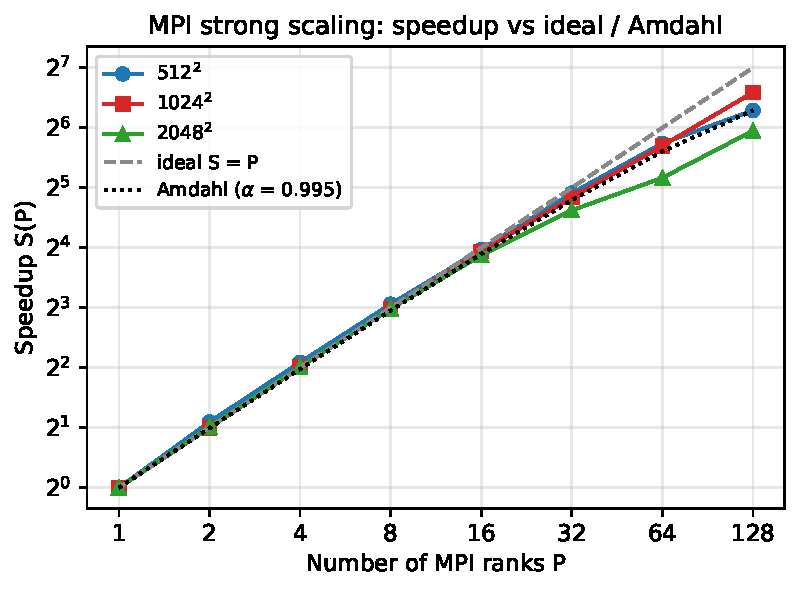
\includegraphics[width=\columnwidth]{mpi_strong_speedup.pdf}
  \caption{MPI strong scaling: measured speedup $S(P)=\mathrm{MLUPS}(P)/
  \mathrm{MLUPS}(1)$ for three grid sizes, with the ideal line $S=P$ and
  an Amdahl prediction ($s=0.005$). The deviation at high $P$ is caused
  by communication and bandwidth, not by a serial fraction.}
  \label{fig:strong-speedup}
\end{figure}

\paragraph{The crossover (a richer reading).} Fig.~\ref{fig:strong-eff}
plots the efficiency $E(P)=S(P)/P$ and tells a more interesting story
than ``bigger scales better''. At low $P$ we see \textbf{super-linear
speedup} ($E>100\%$) for $512^2$ and $2048^2$: as the subdomain shrinks
it starts to fit in cache, so each core runs faster per cell than the
$P=1$ run did. This is a cache effect, not an error. At high $P$ two
\emph{opposite} limiters
appear. The small grid ($512^2$) becomes \textbf{communication-bound}:
at $P=128$ each rank owns only four rows but still exchanges two, so
efficiency collapses to $61\%$. The large grid ($2048^2$) becomes
\textbf{memory-bandwidth-bound}: its subdomains never fit in cache, and
packing many cores on one node saturates the shared memory bus, which
already drops efficiency to $56\%$ at $P=64$ \emph{within one node}.
The middle size $1024^2$ is the \textbf{sweet spot} ($75\%$ at $P=128$):
large enough to keep communication small, small enough to get some cache
benefit. So the idea that ``a bigger grid always scales better'' is only half
true: it holds up to $1024^2$, but $2048^2$ is limited by memory bandwidth
rather than communication, so it is actually the worst at high $P$.

\begin{figure}[t]
  \centering
  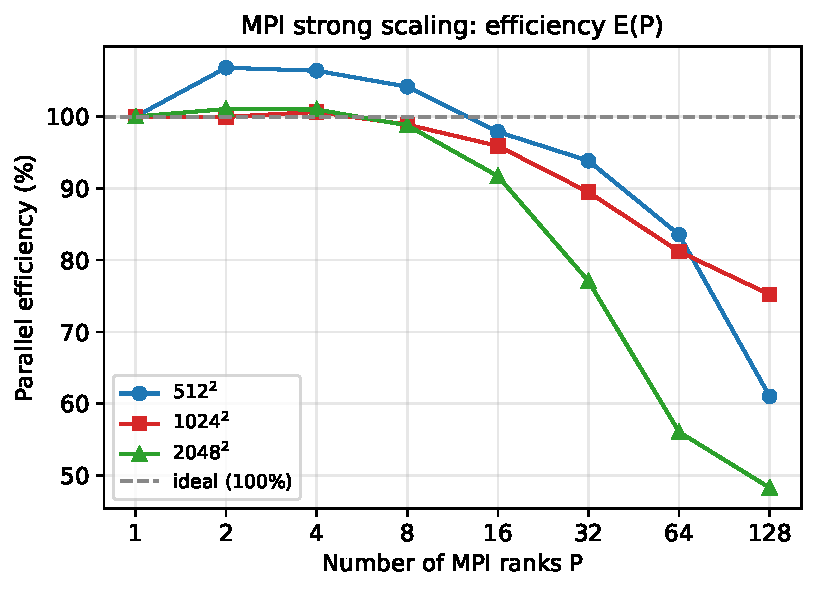
\includegraphics[width=\columnwidth]{mpi_strong_efficiency.pdf}
  \caption{MPI strong scaling: efficiency $E(P)$ for three sizes. Note
  the super-linear region ($E>100\%$, cache), and the crossover at high
  $P$: $512^2$ is communication-bound, $2048^2$ is bandwidth-bound, and
  $1024^2$ is the best compromise.}
  \label{fig:strong-eff}
\end{figure}

\paragraph{Weak scaling vs Gustafson.} We keep the per-rank work
constant (128 rows/rank, $n_x=1024$, $n_y=128P$). Gustafson's law with a
tiny $s$ predicts nearly flat efficiency. Fig.~\ref{fig:weak} shows the
efficiency falling from $100\%$ to $39\%$ over $P=1\ldots128$, which we
explain by three distinct causes visible on the curve. (1) The
$P{=}1\!\to\!2$ step is mainly a cache effect, not communication: the small
per-rank domain lets the $P=1$ point sit in the shared L3 cache (28.6 MLUPS
vs only $\sim$21 for the strong $P=1$ runs), an advantage lost once two cores
share that L3 at $P=2$. (2) The gradual decline on a single node
($P=8\ldots64$): \textbf{shared memory-bandwidth saturation} as the node
fills, the dominant limiter for this memory-bound code, and \emph{not}
the communication, which is nearest-neighbour and constant per rank.
(3) The sharp drop at $P=128$: crossing onto a \textbf{second node}
(inter-node network) once the first 72 cores are full. Throughput still
grows from 28.6 to 1434 MLUPS, so weak scaling works; the loss is fully
explained.

\begin{figure}[t]
  \centering
  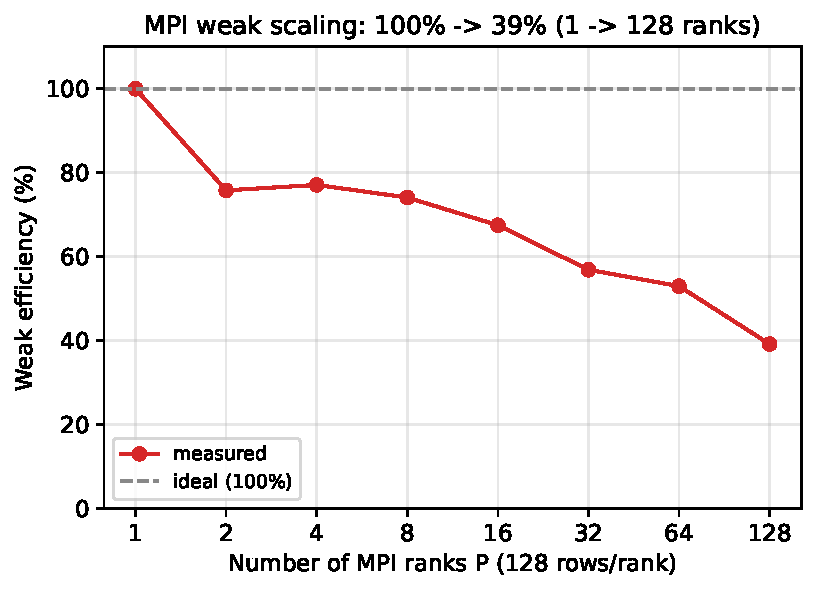
\includegraphics[width=\columnwidth]{mpi_weak.pdf}
  \caption{MPI weak scaling efficiency (128 rows/rank). The drop combines the
  loss of the cache-boosted $P=1$ baseline, intra-node bandwidth saturation,
  and the inter-node step at $P>72$.}
  \label{fig:weak}
\end{figure}

% =====================================================================
\section{CUDA version}
% =====================================================================
\paragraph{Design.} On a single GPU the whole grid lives in one memory,
so there is \textbf{no communication at all}. The natural mapping is
\textbf{one thread per cell}, with one kernel per phase
(collide, bounce-back, stream, inlet, outlet) launched in order in the
default stream, so each kernel sees the previous one's result without an
explicit synchronisation. Streaming uses \textbf{double buffering}: the
kernel reads \texttt{d\_f} and writes \texttt{d\_ftmp}, then we swap the
two device pointers on the host (no copy), the GPU equivalent of the
serial \texttt{f.swap(ftmp)}. The small read-only tables $c_x,c_y,w$ live
in \texttt{\_\_constant\_\_} memory. Host$\leftrightarrow$device copies
happen \textbf{only at init and once at the end}; the probe is accumulated
on the device and copied back once, so nothing crosses the bus inside the
hot loop and the timing stays clean. The
CUDA version reproduces $St=0.1600$ and reaches \textbf{2051 MLUPS} on a
V100, about $\mathbf{101\times}$ the serial baseline.

\paragraph{Roofline.} LBM has low arithmetic intensity, so it is
\textbf{memory-bandwidth bound}. Per cell per step the unavoidable
traffic is roughly $36$ doubles $=288$ bytes (collide and stream each
read and write nine doubles). With the V100 peak bandwidth $\sim900$
GB/s, the ceiling is
\begin{equation}
  \mathrm{MLUPS}_{\max}\approx \frac{900\times10^9}{288}\approx 3100.
\end{equation}
The reference run reaches $2051/3100\approx66\%$ of this bound. We are
\emph{below} the ceiling, so there is no measurement anomaly (a value
above $\sim3100$ would have signalled an error). The remaining gap is the
expected mix of imperfect coalescing, the cheap extra kernels and the
per-step launch overhead.

\paragraph{Study: block, size, layout.} We sweep three parameters at
fixed throughput. The \emph{block size} gives a broad plateau between 128
and 512 threads ($\sim2300$ MLUPS); only $32$ (a single warp) is clearly
worse, because there are too few warps to hide memory latency. For a
memory-bound kernel the block size mostly changes occupancy, not the
ceiling. The \emph{problem size} sweep rises from 1940 MLUPS at $512^2$ to
2513 at $4096^2$ ($\sim81\%$ of the roofline), because larger grids
amortise the fixed per-step costs (five kernel launches, the
single-thread inlet/outlet/probe kernels) over more cells. The
\emph{memory layout} is the headline (Fig.~\ref{fig:cuda-layout}):
\textbf{SoA is $\mathbf{3.6\times}$ faster than AoS}. With SoA
($f[i\,N+k]$) consecutive threads read consecutive addresses, so a warp's
loads \textbf{coalesce} into a few wide transactions. With AoS
($f[k\,Q+i]$) the nine directions of a cell are packed together, so
consecutive threads are nine doubles apart, the loads scatter across many
cache lines, and most of every fetched line is wasted. Same arithmetic,
same logical bytes; only the access pattern changes, and for a
memory-bound code the access pattern is everything. This is why SoA was
chosen from the start.

\begin{figure}[t]
  \centering
  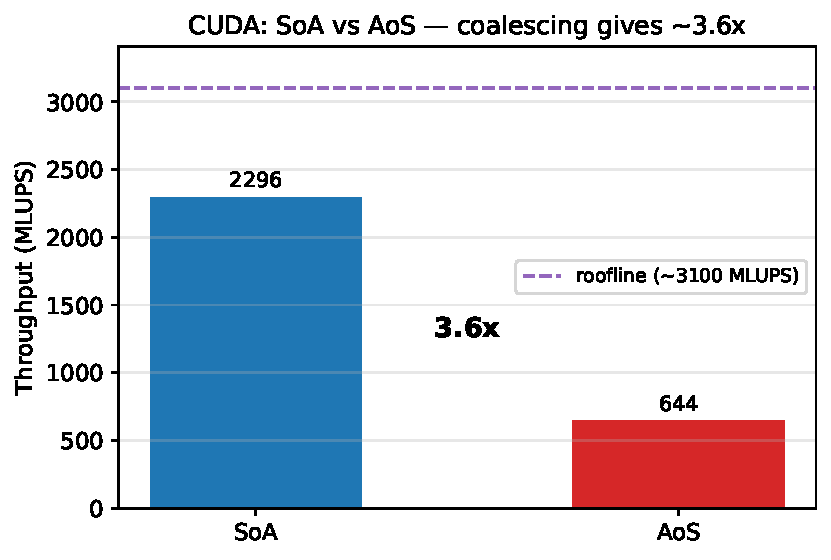
\includegraphics[width=\columnwidth]{cuda_layout.pdf}
  \caption{CUDA memory layout at $1024^2$: SoA reaches $\sim74\%$ of the
  $\sim3100$ MLUPS roofline while AoS collapses to $\sim21\%$, a
  $3.6\times$ gap caused purely by memory coalescing.}
  \label{fig:cuda-layout}
\end{figure}

% =====================================================================
\section{Conclusion}
% =====================================================================
Both parallel versions reproduce the correct physics ($St=0.16$). The MPI
version reaches $\sim99\%$ efficiency on one node and scales to 128 ranks,
with a clear, hardware-level explanation of the deviations:
communication for small grids, bandwidth for large grids, and a step
beyond one node. The CUDA version runs $\sim101\times$
faster on a single V100 and sits at a steady fraction of the
roofline, with memory coalescing (SoA vs AoS,
$3.6\times$) as the single most important lesson. In both cases the
limiter is memory traffic, not arithmetic, which is the expected
behaviour for a stencil code with low arithmetic intensity.

% =====================================================================
\section*{AI usage statement}
% =====================================================================
\small
I used an AI assistant (Anthropic Claude) throughout this project. It
helped me design and write large parts of the MPI and CUDA code (the
1D decomposition, the halo exchange, the CUDA kernels and double
buffering), set up the Slurm scripts and the plotting pipeline, and draft
this report and the slides (it mainly generated the template and
rephrased my sentences). I checked its output myself: I built and ran
every version on the SCITAS clusters, validated the physics with the
provided \texttt{strouhal.py} ($St=0.16$ in all cases), verified that the
MLUPS definition is identical across versions, and confirmed that all
measured throughputs stay below the V100 bandwidth roofline. I kept a
logbook of the main choices along the way, and I made sure I understand
how each part it wrote works and checked whether it matched my
instructions.

\end{document}
